\documentclass{article}
\usepackage{enumitem,amssymb}
\newlist{todolist}{itemize}{2}
\setlist[todolist]{label=$\square$}
\usepackage{hyperref}
\hypersetup{
	colorlinks=true,
	linkcolor=blue,
	filecolor=magenta,      
	urlcolor=cyan,
	pdftitle={Overleaf Example},
	pdfpagemode=FullScreen,
}
\usepackage{graphicx}
\usepackage[margin=0.75in,headsep=.2in]{geometry}


\usepackage[svgnames,table]{xcolor}
\usepackage[tableposition=above]{caption}
\usepackage{pifont}

\newcommand*\CHECK{\ding{51}}

\begin{document}
	
{\huge \textbf{Kinetic Systems Class VERSIONNUMBER}}

\vspace{1cm}

{\huge \textbf{Vocabulary Sheet}}

\begin{itemize}
  \item \textbf{Git} - A Version Control System for managing text files
  \item \textbf{GitHub} - A website where git repositories are shared
  \item \textbf{Repository} - A collection of files and their save-points
  \item \textbf{Github Project} - A collection of repositories 
  \item \textbf{Repository Fork} - A copy of a repository that you can edit
  \item \textbf{Pull Request} - A request to bring changes from a forked repository into the origin
  \item \textbf{Github Issue} - A task in the TODO list within Github
  \item \textbf{Linux } - An operating system for most computers in the world
  \item \textbf{Arduino } - A tool chain for programming micro-controllers 
\end{itemize}

\newpage
\section{Introduction And Software Tools:}
\begin{todolist}
	\item Create Github Account
	\item Install Arduino
	\item Introduce Arduino Uno Board
	\item Introduce Examples
	\item Run Blink
\end{todolist}


\section{Circuits, Servos and Github:}
\begin{todolist}
	\item Breadboard an LED circuit
	\item Change LED circuit to connect to Arduino
	\item Breadboard a Servo circuit
	\item Run Servo Sweep example
\end{todolist}

\section{Potentiometers and Resistors:}
\begin{todolist}
	\item Breadboard a pot circuit
	\item Run the pot read example
	\item Open Serial Monitor and see print statements
	\item Read Arduino map() reference
	\item Use pot to control servo
\end{todolist}


	
\section{Github and Issues:}
\begin{todolist}	
	\item Install Github Desktop
	\item Introduce Github Issues
	\item Add students to Github Project
	\item Create a .ino file with blink and sweep
	\item Commit with issue number linking
	\item Push changes to close issue
	\item Make issue to control servo with potentiometer
	\item Commit to close issue and push
\end{todolist}

\newpage	
\section{CAD, Tinkercad and STL's:}
\begin{todolist}
	\item Install Cura 5.4+	
	\item Go to Tinkercad.com and make an account with your Bancroft Gmail
	\item Follow the Make a Nametag worksheet
	\item Open Nametag STL in Cura
	\item Slice and view layers in Cura
	\item Submit STL to Google Drive for printing
\end{todolist}

\section{BowlerStudio Intro:}
\begin{todolist}
	\item Install BowlerStudio
	\item Discuss What is Programmatic CAD
	\item Discuss Programmatic CAD vs Sketch->extrude paradigm
	\item Run Text to Speech Example
	\item Make a copy and modify example
	\item Run modified example
	\item Publish with commit message
	\item Make a new project in BowlerStudio called "ScriptTest"
	\item Make a file called ScriptTest and select groovy as type
	\item Print "Hello world" to the terminal
	\item Commit and push
	\item Go to GitHub.com to verify
\end{todolist}

\newpage

\section{CAD, BowlerStudio and Releases:}
\begin{todolist}
	\item Make an Issue to add a Nametag script
	\item Add a file to git repo in BowlerStudio
	\item Use Text extrude to add name
	\item Use getTotalX() and getTotalY() to add a backing plate with 2mm boarder
	\item Commit to close Issue
	\item Make a Release and watch the STL creation in CI
	\item Make issue to add servo and wave name
	\item Add a Servo and Servo Horn vitamin from menu
	\item Cut horn from nametag
	\item Make a block and cut servo from it
	\item Give all parts names and layout a print bed
	\item Commit to close issue
	\item Make Second release with servo assembly
	\item Make an Issue to add assembly steps
	\item Add an assembly step for each part
	\item Commit to close the issue and push
	\item Make a Third release
\end{todolist}
\newpage
\section{Kinematics To CAD linking:}
\begin{todolist}
	\item Discuss a 1 DOF "arm"
	\item Attach CAD to kinematics
	\item Pass the link length to the cad script
	\item Move cad elements based on kinematic configuration [simple]
	\item Introduce Transform Objects
	\item Move cad elements based on kinematic configuration [Transform]
	\item Convert CAD script into an object
	\item Convert CAD script to take Transform to generate links
	\item Convert CAD script to take Transform and next Link Motor
\end{todolist}

\section{Kinematics Solving: Analytic Solution}
\begin{todolist}
	\item Forward Kinematics of a 1dof [sin and cos]
	\item Inverse Kinematics of a 1 dof [atan2]
	\item Forward Kinematics of a 2 dof [sin and cos ]
	\item Inverse kinematics of a 2 dof [ Law of Cosines] 
\end{todolist}
\section{Forward Kinematics with D-H parameters:}
\begin{todolist}
	\item Discuss a frame transformation
	\item Discuss inverting frame transformations
	\item Use transformations to move cubes
	\item Introduce Denavit Hartenberg Notation for defining Links
	\item Watch  \url{https://www.youtube.com/watch?v=nuB_7BkYNMk}
	\item Solve Forward Kinematics using D-H convention
\end{todolist}

\section{Inverse Kinematics with D-H parameters:}
\begin{todolist}
	\item Discuss a 3 dof arm/leg
	\item Solve Inverse Kinematics using D-H convention
	\item Use transform inversions to set up the triangle 
	\item Solve using law of cosine on alligned triangle
\end{todolist}


\section{BowlerStudio Creatures:}
\begin{todolist}
	\item Open SmallKat Marcos
	\item Follow Tutorial steps 1-3:  \url{http://commonwealthrobotics.com/Mobile-Base-Control/BasicWalking/}
	\item Use a transformation as a body pose, see  \url{https://youtu.be/FPDERQYFSFY}
\end{todolist}


\section{Bonus Month, BowlerStudio Design Challenge:}
\begin{todolist}
	\item Make a Copy of SmallKat Marcos
	\item Load the STL of the head and modify it
	\item Design a head based on Spike
	\item attach Spike head to neck base
	\item Print and verify new head works with SmallKat
\end{todolist}

\newpage

\leftline{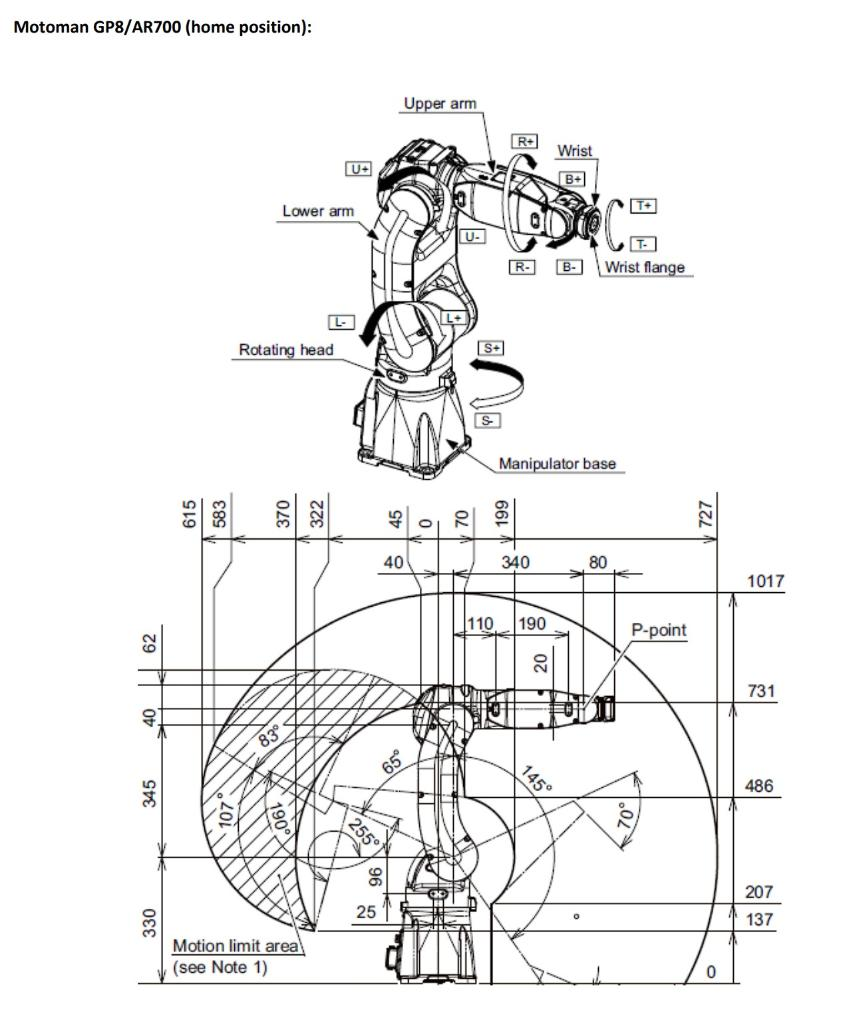
\includegraphics[scale=0.5]{robotarm.jpeg} }

\begin{table}
	\caption{Write the D-H parameters for this robot}
	\rowcolors{1}{}{gray!7}
	\begin{tabular}[t]{lccccccc}
		Link & Theta & D 	  & Radius & Alpha \\ 
		S 	 & 	     &        &        &       \\	
		L 	 & 	     &        &        &       \\	
		U 	 & 	     &        &        &       \\	
		R 	 & 	     &        &        &       \\	
		B 	 & 	     &        &        &       \\	
		T 	 & 	     &        &        &       \\	
	\end{tabular}
\end{table}
\newpage

\end{document}
